%!TEX root = TQFTnotes.tex
%%%%%%%%%%%%%%%%%%%%%%%%%%%%%%
\chapter{Classification of 2d TQFT}\label{c:2d-classification}
In this chapter, we present a full classification of 2-dimensional TQFTs; the
final answer, given in \thref{t:2d-classification2}, states that such theories
are classified by commutative Frobenius algebras. This is a relatively simple
result; it goes back to at least 1989, see Dijkgraaf's thesis
\cite{dijkgraaf-thesis}, but was probably known to experts much earlier. For
us, it will serve as a model example for all future constructions.

For a two-dimensional TQFT, there is only one $1$-dimensional oriented closed
manifold: the circle $S^1$, and any orientation-preserving diffeomorphism
$S^1\to S^1$ is isotopic to the identity. It also seems obvious (and in fact
can be justified using Morse theory, as we discuss below)  that any
cobordism can be obtained by gluing pieces diffeomorphic to one of the
cobordisms below together with the cylinder $S^1\times I$:
\begin{center}
  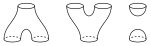
\includegraphics{figures/c4-fig01.svg}
\end{center}

It is also not hard to write some relations, such as the
associativity relation

\begin{equation}\label{e:2d-assoc-prelim}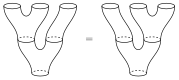
\includegraphics{figures/c4-fig02.svg}\end{equation}


However, how can one show that this is the full list of relations?

There are two approaches. One, used in \cite{kock}, uses the classification of
surfaces; using that, we show that the relations we have are enough to bring any
composition of generators to some canonical form. This approach does not require
much beyond the classification of surfaces, but it does not generalize to
higher dimensions.

There is, however, an alternative approach, based on Morse and Cerf theory.
This goes back at least to \cite{abrams}, who used a handle-decomposition
viewpoint to give a classification of 2d TQFTs; the Cerf-theoretic version
is presented in \cite{moore-segal} and \cite[Lecture~23]{freed-bordism},
the latter of which our exposition follows. One can also find more details
in the unpublished paper \cite{gay-wehrheim-woodward}.

%%%%%%%%%%%%%%%%%%%%%%%%%%%%%%
\section{Morse theory basics}\label{s:morse}

We start with an overview of Morse theory; details can be found, e.g., in
\cite{matsumoto}.

Recall that given a smooth real-valued function $f$ on an $n$-dimensional
manifold $M$, a point $p\in M$ is a \emph{non-degenerate critical point}
\index{critical point!non-degenerate} if
$\del_i f (p)=0$ and the Hessian matrix
$a_{ij}=\frac{\del^2 f}{\del  x^i \del x^j}(p)$ is non-degenerate. It is easy to
see that this is independent of the choice of coordinate system. It is also
known that in such a case, one can choose local coordinates in a neighborhood
of $p$ so that
\begin{equation}\label{e:crit-point}
  f(x^1, \dots, x^n)=c-(x^1)^2 -\dots -(x^r)^2
  + (x^{r+1})^2+ \dots + (x^n)^2
\end{equation}
(this statement is usually called the \emph{Morse lemma}\index{Morse lemma}).
The number $r$ of minuses in \eqref{e:crit-point} is called the \emph{index}
of the critical point.

It is immediate from the definition that a non-degenerate critical point
is isolated; thus, if $M$ is compact, there can be only finitely many
non-degenerate critical points.

\begin{definition}\label{d:morse_function}\index{Morse function}
  Let $M$ be a closed $n$-manifold. A Morse function is a
  smooth function $f\colon M\to \R$ such that all critical points
  of $f$ are non-degenerate.
\end{definition}

It will be more useful to impose a stronger condition.

\begin{definition}\label{d:morse_function2}
  Let $M$ be a closed $n$-manifold. A Morse function  $f\colon M\to \R$
  is called \emph{excellent}\index{Morse function!excellent} if all critical
  values $c_i=f(p_i)$ are distinct.
\end{definition}

It was proved by Morse that such functions exist; moreover, the set $\calF^0$
of excellent functions is an open and dense subset in $C^\infty(M)$
(in an appropriate topology).

We can generalize the notion of excellent functions to manifolds with boundary,
or to cobordisms $N_0\cob{M} N_1$.

\begin{definition}\label{d:morse-function3}
  Let $N_0\cob{M} N_1$ be an $n$-dimensional cobordism. A Morse function on $M$
  is a smooth function $f\colon M\to \R$ such that
  \begin{itemize}
    \item $f$ is constant on both in-boundary and out-boundary:
      $f|_{N_0}=a_0=\min_M f$, $f|_{N_1}=a_1=\max_M f$
    \item All critical points of $f$ are in the interior
      $M\setminus (N_0\cup N_1)$, and all critical points are non-degnerate.
  \end{itemize}
  If, in addition, all critical values of $f$ are distinct, then $f$ is called
  \emph{excellent}.
\end{definition}
 Again, one can prove
that such functions exist and form an open dense subset of all functions
satisfying $f|_{N_0}=a_0$, $f|_{N_1}=a_1$.

The main result of Morse theory is that given an excellent function $f$, the
topology of the manifold $M_t=f^{-1}((-\infty, t])$ does not change between
critical values: if $c_i<c_{i+1}$ are critical values, with no other critical
values between them, then for all $t\in I=[c_i+\eps, c_{i+1}-\eps]$, the
manifolds $M_t$ are diffeomorphic, and $M_I=f^{-1}(I)\isoto N_{t_0} \times I$,
where $N_{t_0}=f^{-1}(t_0)$ is a slice for any $t_0\in I$. Moreover, one can
give an explicit description of how topology of $M_t$ changes when one  goes
through a critical point (this is usually referred to as ``attaching a
handle''). In particular, this implies that if $f$ has no critical points, then
$M$ is a cylinder: $M\isoto N\times I$.

Therefore, one can use Morse functions to decompose a cobordism as a
composition of ``elementary'' cobordisms.
\begin{definition}\label{d:elem-cobordism}\index{elementary cobordism}
  An elementary cobordism is a cobordism that admits a Morse  function
  with a single  critical point.
\end{definition}

Thus, given an excellent function with critical values $c_1<\dots<c_k$,
and values on the boundary $f|_{N_0}=a_0<c_1$, $f|_{N_1}=a_k>c_k$, we
can choose intermediate values $a_i\in (c_i, c_{i+1})$; then we have
\begin{equation}\label{e:morse-decomposition}
  M=M_k\circ \dots \circ M_1,
\end{equation}
where $M_i=f^{-1}([a_{i-1}, a_i])$ is the elementary cobordism containing
critical point $p_i$. It follows from the result above that up to
isomorphism, $M_i$ does not depend on the choice of $a_i$. We will refer to
\eqref{e:morse-decomposition} as a
\emph{Morse decomposition}\index{Morse decomposition} of a cobordism.

In particular, for $n=2$, each connected elementary cobordism is isomorphic to
one of the four cobordisms shown in Table~\ref{tab:elementary-2cob}. Note that
here we follow our convention that cobordisms go ``top to bottom''; thus, the
$y$-axis is directed downward, so that the minimal value of $f$ is at the top,
and the maximal, at the bottom.
\begin{table}[ht]
  \centering
  \setlength{\extrarowheight}{8pt}%
  \begin{tabular}{|l|l|}
    \hline
    Index  & Elementary cobordism \\
    \hline
    0 &
    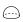
\includegraphics{figures/c4-fig03.svg} \\[8pt]
    \hline
    1 &
    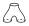
\includegraphics{figures/c4-fig04.svg} \qquad
    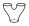
\includegraphics{figures/c4-fig05.svg} \\[12pt]
    \hline
    2 &
    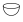
\includegraphics{figures/c4-fig06.svg} \\[8pt]
    \hline
  \end{tabular}
  \medskip
  \caption{Connected elementary $2$-cobordisms}
  \label{tab:elementary-2cob}
\end{table}
A (not necessarily connected) elementary cobordism is obtained as a disjoint
union of one of the connected elementary cobordisms and  several copies of the
identity cobordism, i.e., $S^1\times I$.

Thus, we see that a choice of an excellent function gives a presentation of a
2-cobordism as a composition of the generators shown in
Table~\ref{tab:elementary-2cob} (and identity cobordisms).

%%%%%%%%%%%%%%%%%%%%%%%%%%%%%%%%%%%%
\section{Cerf theory}\label{s:cerf}

We have seen that excellent Morse functions allow one to present a cobordism as
a composition of elementary cobordisms; for $n=2$, this gives us a set of
generators for the category of cobordisms.



To describe relations between generators, we need to see how one can go from
one such presentation to another, or equivalently, how the presentation changes
if we replace one excellent Morse function by another.

It is easy to see that the space of excellent functions is not connected; thus,
if $f_0$, $f_1$ are two excellent functions, and we want to connect them by a
path $f_s$, $s\in [0,1]$ in the space of functions, in general this path must go
through some points which are not excellent. This was studied by Cerf in
\cite{cerf} and is usually referred to as \emph{Cerf theory}\index{Cerf
theory}.

\begin{example}\label{x:morse-x3}
  Consider the one-parameter family of functions $f_s= x^3+sx$ on a neighborhood
  of the origin in $\R$, with local coordinate $x$, shown in \firef{fig:x3}.

  Then for $s<0$, the function is Morse with two critical points of indices
  $0$ and $1$ respectively; for $s>0$, it is also Morse, with no critical
  points; and for $s=0$, $f_0(x)=x^3$ is not a Morse function: zero is a
  degenerate critical point. Thus, in this case, $f_s$, considered as a path in
  the function space, connects two Morse functions but goes through a non-Morse
  function $f_0=x^3$. This path describes annihilation of a pair of critical
  points (or, going in the opposite direction, birth of a pair of critical
  points).

  \begin{figure}[ht]
    \centering
    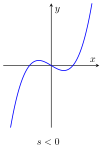
\includegraphics{figures/c4-fig07.svg}
    \qquad
    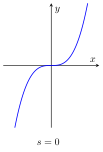
\includegraphics{figures/c4-fig08.svg}
    \qquad
    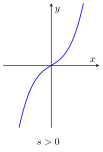
\includegraphics{figures/c4-fig09.svg}
    \caption{Birth-death of critical points in family  $f_s=x^3+sx$}
    \label{fig:x3}
  \end{figure}


\end{example}

\begin{example}\label{x:morse-crossing}
  Consider the family of  functions $f_s(x)=x^2-x^4+sx$. Then for values of $s$
  close to 0, it has three  critical points, all of them non-degenerate: local
  minimum at $p_0$ close to 0, and local maxima at points $p_1<0$, $p_2>0$.

  For $s<0$, we have $c_1>c_2$; for $s>0$, $c_1<c_2$, and for $s=0$, $c_1 = c_2$
  as shown below, so for $s=0$ this function is Morse but not excellent. Thus,
  we again get a path connecting two excellent functions going through a
  non-excellent function with $c_1=c_2$.

  \begin{figure}[ht]
    \centering
    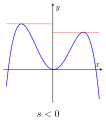
\includegraphics{figures/c4-fig10.svg}
    \qquad
    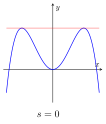
\includegraphics{figures/c4-fig11.svg}
    \qquad
    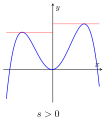
\includegraphics{figures/c4-fig12.svg}

    \caption{Crossing of critical values in family $f_s=x^2-x^4+sx$}
    \label{fig:x4-x2}
  \end{figure}

\end{example}

It turns out that these two model examples are enough: any two excellent
functions can be connected by a one-parameter family where all non-excellent
functions are at worst as in these examples. More precisely, we have the
following.

\begin{definition}\label{d:morse-good}
  A \emph{good}  function on an $n$-dimensional closed manifold $M$ is a
  smooth function of one of the following types:
  \begin{itemize}
    \item {\bf Type $\alpha$}: all critical values are distinct, and all
      critical points are non-degenerate, except for one. Near this point,
      there is a local coordinate system where $f$ is given by
      $$
      f(x^1, \dots, x^n)=c+(x^1)^3 -(x^2)^2-\dots -(x^r)^2+(x^{r+1})^2 +
                        \dots +(x^n)^2.
      $$
    \item {\bf Type $\beta$}: all critical points are non-degenerate, and
      all critical values are distinct except for one pair: $c_i = c_j$
      for some $i\ne j$.
  \end{itemize}
  In a similar way one defines good function on a cobordism $M$.
\end{definition}

(The name ``good'' is not standard.)

It was shown by Cerf that this is the beginning of a stratification of the
space $\calF=C^\infty(M)$: we can write
$\calF = \calF^0\sqcup \calF^1\sqcup\dots$,
where $\calF^0$ is the set of excellent functions, which is open and dense in
$\calF$; the set $\calF^1$ consists of good functions and is a codimension 1
subset of $\calF$, and so on. (One can also define higher codimension strata,
but we will not need them.) A review of this theory can be found, e.g., in
\cite[Section I.2]{hatcher-wagoner}.

\begin{theorem}\label{t:cerf1}
  Let $f_0, f_1$ be two excellent functions on a cobordism $M$. Then one can
  find a one-parameter family $f_s$ of smooth functions on $M$ such that:
  \begin{enumerate}
    \item $f_s$ is excellent for all $s$ except for finitely
      many values $s_1, \dots, s_p$
    \item At each of these special values, $f_s$ is good.
  \end{enumerate}
\end{theorem}
In other words, any two points in $\calF^0$ can be connected by a path
contained in $\calF^0\cup \calF^1$.

Moreover, this path can be chosen so that it is transversal to $\calF^1$ (we
skip the precise definition, referring the reader to \cite{hatcher-wagoner}).
This allows one to describe how the Morse decomposition changes when we cross
one of the components of $\calF^1$ (``walls''). Crossing a component
corresponding to a type-$\alpha$ function produces a \emph{birth-death move}:
two adjacent critical points (of indices $r-1, r$) appear or disappear.
Crossing a component corresponding to a type-$\beta$ function produces a
\emph{crossing move}: two critical values $c_i, c_{i+1}$ exchange their order.

\begin{theorem}\label{t:cerf}
  Let $M$ be a cobordism, and let $f_0, f_1$ be two excellent functions on
  $M$, with corresponding Morse decompositions $\calD_0$, $\calD_1$ as in
  \eqref{e:morse-decomposition}. Then $\calD_0$ and $\calD_1$ can be obtained
  from each other by a finite sequence of birth-death moves and crossing
  moves and their inverses.
\end{theorem}


%%%%%%%%%%%%%%%%%%%%%%%%%%%%%%%%%%%%%%%%
\section{Generators and relations of $\twoCob$}\label{s:2cob-relations}

Now let us apply the general theory above to the question of classification
of 2d TQFTs.

First, choosing an excellent Morse function on a 2d cobordism $M$, we get a
decomposition of $M$ into a composition of elementary cobordisms. Each elementary
cobordism is a disjoint union of copies of the connected elementary cobordisms;
and each connected elementary cobordism is isomorphic to one of the standard
cobordisms shown in Table~\ref{tab:elementary-2cob}: pair of pants, copants,
cap, and cup.

Let us denote by $A=Z(S^1)$ the vector space associated to the circle, and by
$m, i, \Delta, \eps$ the linear operators corresponding to the standard
cobordisms as shown below.

\begin{equation}\label{e:frobenius-data}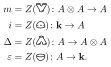
\includegraphics{figures/c4-eqfig01.svg}\end{equation}


Then a choice of an excellent Morse function $f$ on $M$, together with a choice
of isomorphism $\ph_i$ of each of the connected elementary cobordisms defined by
$f$ with one of the ``standard'' ones, gives us a presentation of $Z(M)$ as a
composition of tensor products of operators $m, i, \Delta, \eps$
(and the identity operator $\id_A$).
Therefore, the structure of TQFT is completely determined by these 4 operators.
Note also that $m$ and $\Delta$ are symmetric: $m\circ P= m$, where
$P\colon A\otimes A\to A\otimes A$ is the permutation
$P(a\otimes b)= b\otimes a$. Indeed, this follows from the isomorphism of
cobordisms shown below: the standard copants surface admits a self-diffeomorphism
(a $180^\circ$ rotation about its central vertical axis) that swaps the two
input boundary circles and fixes the output boundary circle.
\begin{equation}\label{e:m-symmetric}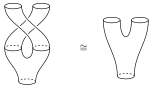
\includegraphics{figures/c4-fig13.svg}\end{equation}
The analogous argument applied to the pants surface (turn the picture upside
down) gives $P\circ\Delta = \Delta$.

Next, observe that the choice of isomorphisms $\ph_i$ is in fact irrelevant.
Indeed, since any orientation-preserving diffeomorphism $\ph$ of $S^1$ is
isotopic to the identity, by \leref{l:tqft-isotopy} its action on $A$ is trivial:
$\ph_*=\id_A$. From this it immediately follows that if $M$ is topologically a
disk, considered as a cobordism $\varnothing \cob{} S^1$ (i.e., a cap), then the
operator $Z(M)\colon \kk \to A$ does not depend on the choice of the isomorphism
of $M$ with the standard cap; a similar result holds for the cup.

If $M$ is a cobordism $S^1\sqcup S^1\to S^1$ which is isomorphic to the
standard pair of pants, there are just two isomorphisms up to isotopy; one is
obtained from the other by composing with the diffeomorphism that interchanges
the two circles that form the in-boundary. But since $m$ is symmetric as
discussed above, both choices of isomorphism give us the same operator
$Z(M)=m\colon A\otimes A\to A$. A similar statement holds for the cobordism
$S^1\cob{} S^1\sqcup S^1$.

Summarizing, we see that for any cobordism $M$, the presentation of $Z(M)$ as a
composition of tensor products of $m, i, \Delta, \eps$ only depends on the
choice of an excellent Morse function and does not depend on any additional
data.

Thus, to check that $Z(M)$ does not depend on any choices, we need to check
that $Z(M)$ is invariant under the Cerf moves described in \thref{t:cerf}. Let
us analyze what these moves look like for $n=2$.

The birth-death moves (type $\alpha$) are easily seen to be of one of the
following two types:
\begin{center}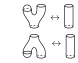
\includegraphics{figures/c4-eqfig02.svg}\end{center}

Now let us consider the crossing move. Assume that we have a family of Morse
functions $f_s$ and two critical points $p_1, p_2$ such that for $s<0$,
$c_1<c_2$, for $s>0$, $c_1>c_2$, and for $s=0$, $c_1=c_2=c$. Choose some
$a_0<c$, $a_1>c$ and consider the (non-elementary) cobordism
$M=f_{0}^{-1}[a_0, a_1]$.

Since operators of the form $X\otimes 1$ and $1\otimes Y$ commute anyway, if
the points $p_1, p_2$ are in different connected components of the cobordism
$M$, then the crossing move does not give any new conditions on
$m, i, \Delta, \eps$.
Therefore, we only need to consider the case when the two critical points $p_1,
p_2$ are in the same connected component of the critical level set
$S=f_0^{-1}(c)$. This immediately implies that each of the critical points is of
index 1.

The set $S$ is a smooth curve except at critical points, where $S$ looks like a
coordinate cross; thus, $S$ is a graph with two 4-valent vertices $p_1$, $p_2$.
Moreover, since $M$ is oriented, we can define an orientation on $S$ (for
example, defining the tangent vector $v$ to $S$ by the condition that $(v, \grad
f)$ is a positively oriented frame). Orientation also gives a cyclic order of
edges at each vertex $p_i$. Using Morse lemma, it is easy to see that
near each critical points $S$ looks as shown below:
\begin{equation}\label{e:S-local}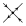
\includegraphics{figures/c4-fig14.svg}\end{equation}

\begin{lemma}\label{l:critical-level}
  Let $S$ be a connected directed graph with two vertices $p_1, p_2$ of degree
  4, together with a cyclic order of edges at each vertex, such that near each
  vertex it is locally isomorphic to the graph shown in \eqref{e:S-local}.

   Then $S$ is isomorphic to one of the four graphs shown in
   \firef{f:critical-level}, and their orientation reversals.
\end{lemma}
The proof of this lemma is an  elementary combinatorics argument; we leave
details  to the reader.


\begin{figure}[ht]
  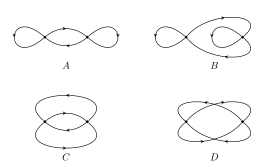
\includegraphics{figures/c4-fig15.svg}
  \caption{Possible shapes of critical level set $S$. Note that for the last
  graph, intersection points are not vertices.}\label{f:critical-level}
\end{figure}


Each of these graphs uniquely determines the corresponding connected component
of the cobordism $M=f_0^{-1}(c-\eps, c+\eps)$; we can recover it by replacing
each arc of the graph by a thin ribbon. For example, for graph A, the
corresponding cobordism is shown below (for reader's convenience, we also show
it in a more familiar form):
\begin{center}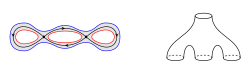
\includegraphics{figures/c4-eqfig03.svg}\end{center}

In this case, one easily sees that the corresponding Cerf move is given by
\begin{center}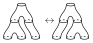
\includegraphics{figures/c4-eqfig04.svg}\end{center}
Reversing the orientation of the graph $A$ is equivalent to flipping the picture
in the vertical direction, which gives the Cerf move below:
\begin{center}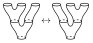
\includegraphics{figures/c4-eqfig05.svg}\end{center}

Similarly, graph $B$ gives the following Cerf move:
\begin{center}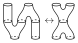
\includegraphics{figures/c4-eqfig06.svg}\end{center}

Graphs $C$ and $D$ are less obvious. For $C$, the cobordism $M$ is of type 2-2:
it is a surface of genus zero, with two circles as in-boundary, and two circles
as out-boundary. However, in this case, the Cerf move looks like:
\begin{center}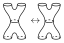
\includegraphics{figures/c4-eqfig07.svg}\end{center}
In other words, both for $s<0$ and for $s>0$ in the family of Morse functions
$f_s$, the corresponding Morse decomposition of the cobordism is a composition
of copants and pants. Thus, it gives no new conditions on $m, \Delta$.

Similarly, graph $D$ gives a cobordism of genus 1 from $S^1$ to $S^1$; again,
in this case both for $s<0$ and for $s>0$ the Morse decomposition looks like

\begin{center}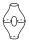
\includegraphics{figures/c4-eqfig08.svg}\end{center}
and thus the corresponding Cerf move gives no new conditions on $m,\Delta$.

Summarising, we see that the non-trivial Cerf moves (both birth-death and
crossings) for $n=2$ are shown in \firef{f:cerf-dim2}. In this table, we also
include the algebraic identities on the operators $m, i, \Delta, \eps$ (defined
by \eqref{e:frobenius-data}) corresponding to each of the moves.

\begin{figure}[ht]
\centering
\renewcommand{\arraystretch}{1.4}
\begin{tabular}{lcl}
  \hline
  \textbf{Name} & \textbf{Cerf move} & \textbf{Algebraic identity}\\
  \hline
  %%%%%%%%%%%%%%%%%%%%%
  Unit &
    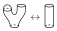
\includegraphics{figures/c4-fig16.svg}
    & $m\circ (i\otimes \id_A) = \id_A$\\[10pt]
  %%%%%%%%%%%%%%%%%%%%%
  Counit &
    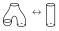
\includegraphics{figures/c4-fig17.svg}
    & $(\eps\otimes \id_A)\circ \Delta = \id_A$\\[10pt]
  %%%%%%%%%%%%%%%%%%%%%
  Associativity &
    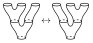
\includegraphics{figures/c4-fig18.svg}
    & $m\circ (m\otimes \id_A) = m\circ (\id_A\otimes m)$\\[20pt]
  %%%%%%%%%%%%%%%%%%%%%
  Coassociativity &
    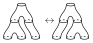
\includegraphics{figures/c4-fig19.svg}
    & $(\Delta\otimes \id_A)\circ \Delta = (\id_A\otimes \Delta)\circ
    \Delta$\\[20pt]
  %%%%%%%%%%%%%%%%%%%%%
  Frobenius &
    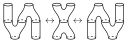
\includegraphics{figures/c4-fig20.svg}
    & $\begin{aligned}
        \Delta\circ m
          &= (m\otimes \id_A)\circ (\id_A\otimes \Delta)\\
          &= (\id_A\otimes m)\circ (\Delta\otimes \id_A)
      \end{aligned}$\\[20pt]
  \hline
\end{tabular}
\caption{Cerf moves in dimension 2 and
         the corresponding algebraic identities}\label{f:cerf-dim2}
\end{figure}

It is easy to see that the identities given by the  unit and associativity moves
are equivalent to the statement that $m, i$ define on $A=Z(S^1)$ a structure of
an associative algebra. Similarly, coassociativity and counit say that $\Delta,
\eps$ define on $A$ a structure of coassocaitive coalgebra.

Combining these identities with the symmetry relations $m\circ P = m$,
$P\circ \Delta = \Delta$ established in \eqref{e:m-symmetric}, we obtain the
following theorem.


\begin{theorem}\label{t:2d-classification}
  A 2d TQFT is equivalent to the following collection of data.
  \begin{itemize}
    \item A vector space $A=Z(S^1)$.
    \item Linear maps $m\colon A\otimes A\to A$, $i\colon \kk\to A$.
    \item Linear maps $\De\colon A\to A\otimes A$, $\eps\colon A\to \kk$.
  \end{itemize}
  This data has to satisfy the following conditions:
  \begin{itemize}
    \item $(A,m, i)$ is a commutative algebra with unit; as usual, we will use
      the notation $ab$ as a shorthand for $m(a\otimes b)$.
    \item $(A,\De, \eps)$ is a cocommutative coalgebra with counit.
    \item The Frobenius condition
      \begin{equation}\label{e:frobenius}
        \De(a_1 a_2) = (a_1\otimes 1) \De(a_2)= \De(a_1)(1\otimes a_2).
      \end{equation}
  \end{itemize}
\end{theorem}

\begin{remark}\label{r:frobenius-two}
  Since $\Delta, m$ are symmetric, any one of the two Frobenius relations
  implies the other; we include both for use in the more general case.
\end{remark}


\begin{remark}\label{r:2d-commutative}
  Note that commutativity of $m$ and cocommutativity of $\Delta$ do not come
  from any of the Cerf moves in \firef{f:cerf-dim2}; they follow from the
  symmetric-pants argument \eqref{e:m-symmetric} (and its mirror image), which
  in turn reflects the symmetric monoidal structure of $\twoCob$.
\end{remark}


A standard way to restate the above theorem is using the notion of Frobenius
algebra.
\begin{definition}\label{d:frobenius}\index{Frobenius algebra}
  A Frobenius algebra is a vector space over a field $\kk$ with two structures:
  \begin{itemize}
    \item A structure of an associative algebra, with multiplication $m$ and
      unit $i\colon \kk \to A$.
    \item A structure of a coassociative coalgebra, with comultiplication $\De$
      and counit $\eps\colon A\to \kk$.
  \end{itemize}
  These two structures must satisfy the Frobenius condition \eqref{e:frobenius}.
\end{definition}
Note that in this definition, we do not assume that $A$ is commutative or
cocommutative.

Then \thref{t:2d-classification} can be rewritten as follows.
\begin{theorem}\label{t:2d-classification2}
  A 2d TQFT is equivalent to a commutative, cocommutative Frobenius algebra.
\end{theorem}
In the next section we will show that cocommutativity follows from
commutativity, so it is enough to require $A$ to be commutative; see
\coref{c:frobenius-commutative}.


\clearpage
